\documentclass{cmspaper}
\usepackage{graphicx}
\renewcommand\arraystretch{1.5}

%%%% needed for the colored notes in the text
%%%% can be removed in final version
\usepackage{color}

\begin{document}

% *** TITLE PAGE ****************************************************************

\begin{titlepage}

% select one of the following and type in the proper number:
% \cmsnote{2008/000}
\internalnote{2009/000}
% \conferencereport{2005/000}
\date{\today}

\title{A Cross-Cleaning Package}

\begin{Authlist}
    Christian~Autermann, Benedikt~Mura, Friederike~Nowak
    \Instfoot{uhh}{Universit\"at Hamburg, Germany}
    Jean-Roch~Vlimant
    \Instfoot{ucsb}{University of California, Santa Barbara, USA}
    % Anyone else ???
\end{Authlist}

% if needed, use the following:
%\collaboration{Flying Saucers Investigation Group}
%\collaboration{CMS collaboration}

%\Anotfoot{a}{On leave from prison}
%\Anotfoot{b}{Now at the Moon}
% if needed, use the following:
%\conference{Presented at {\it Physics Rumours}, Coconut Island, April 1, 2005}
%\submitted{Submitted to {\it Physics Rumours}}
%\note{Preliminary version}

% --- ABSTRACT -----------------------------------------------------------------

\begin{abstract}
Physics analysis in CMS is based on the reconstruction of high-level objects
like electrons, photons, muons, taus, and jets. However, energy depositions in
the detector are not uniquely assigned to one reconstructed physics object but
can contribute to several of them. This leads to an overlap of the objects and
a double counting of energy.

This note discusses a cross-cleaning package which provides algorithms to
identify the overlap of any two objects. The package provides a framework to
correct objects for the double counted energy and to remove duplicates. The
cross-cleaning package is designed to run on {\sc PAT} objects.
\end{abstract} 

% ------------------------------------------------------------------------------

\end{titlepage}

% *** TOC **********************************************************************

\setcounter{page}{2}%JPP
%\tableofcontents

% *** INTRODUCTION *************************************************************

\newpage
\section{Introduction}

In CMS event reconstruction each type of physics object is build from the
detector information by a dedicated algorithm, independent from the
reconstruction of other kinds of objects. It is not uncommon in this procedure
that two or more object of different type end up with common constituents.
While algorithms for object identification usually select 'good' objects
from all reconstructed ones within the same collection, the ambiguity between two
objects in distinct collections can still remain. This multiple counting of
energy must be avoided in order to obtain an optimal energy resolutions of these
objects. This is especially true for the missing transverse energy (MET).

Overlapping objects must be identified and the energy be assigned uniquely to
one of the candidates. The details of such a cleaning are of course depending on
the object definition and therefore particular to each analysis.  In this note a
cross-cleaning package~\cite{package} is discussed, that is flexible enough to
allow the implementation of different splitting algorithm between objects.
If more than two objects share energy, circular dependencies may arise. These
possible interferences are dealt with, so that the outcome of cross-cleaned
objects does not depend on the order in which the cleaning algorithms are
called.

Input to the cleaning are collections of physics objects which pass the
identification requirements chosen for the particular analysis. The
cross-cleaning does not replace a selection on object quality but is meant to
remove the remaining ambiguities.

% *** THE CROSS-CLEANING FRAMEWORK *********************************************

\section{The Cross-Cleaning-Algorithm Framework}
The cross-cleaning is performed in two steps: First binary cleaners are called.
These are specialized algorithms that search for conflicts in two distinct
collections, determine the shared energy for two overlapping objects and decide
how to deal with it. This can for example be an electron-vs.-jet cleaner, a
muon-vs.-jet cleaner etc.. These binary cleaners do not apply any corrections
on either of the two input collections, but save the result of the cleaning
algorithms in an internal map.

The key entry in this map is a reference to the object that should be corrected
or discarded while the associated value contains a vector of objects which are
responsible for this and the information how the object should be corrected. This
scheme is illustrated in Fig.~\ref{fig:Cleaning}. A correction is given by an
energy-momentum fourvector.

% ------------------------------------------------------------------------------
\begin{figure}[hbt]
\begin{center}
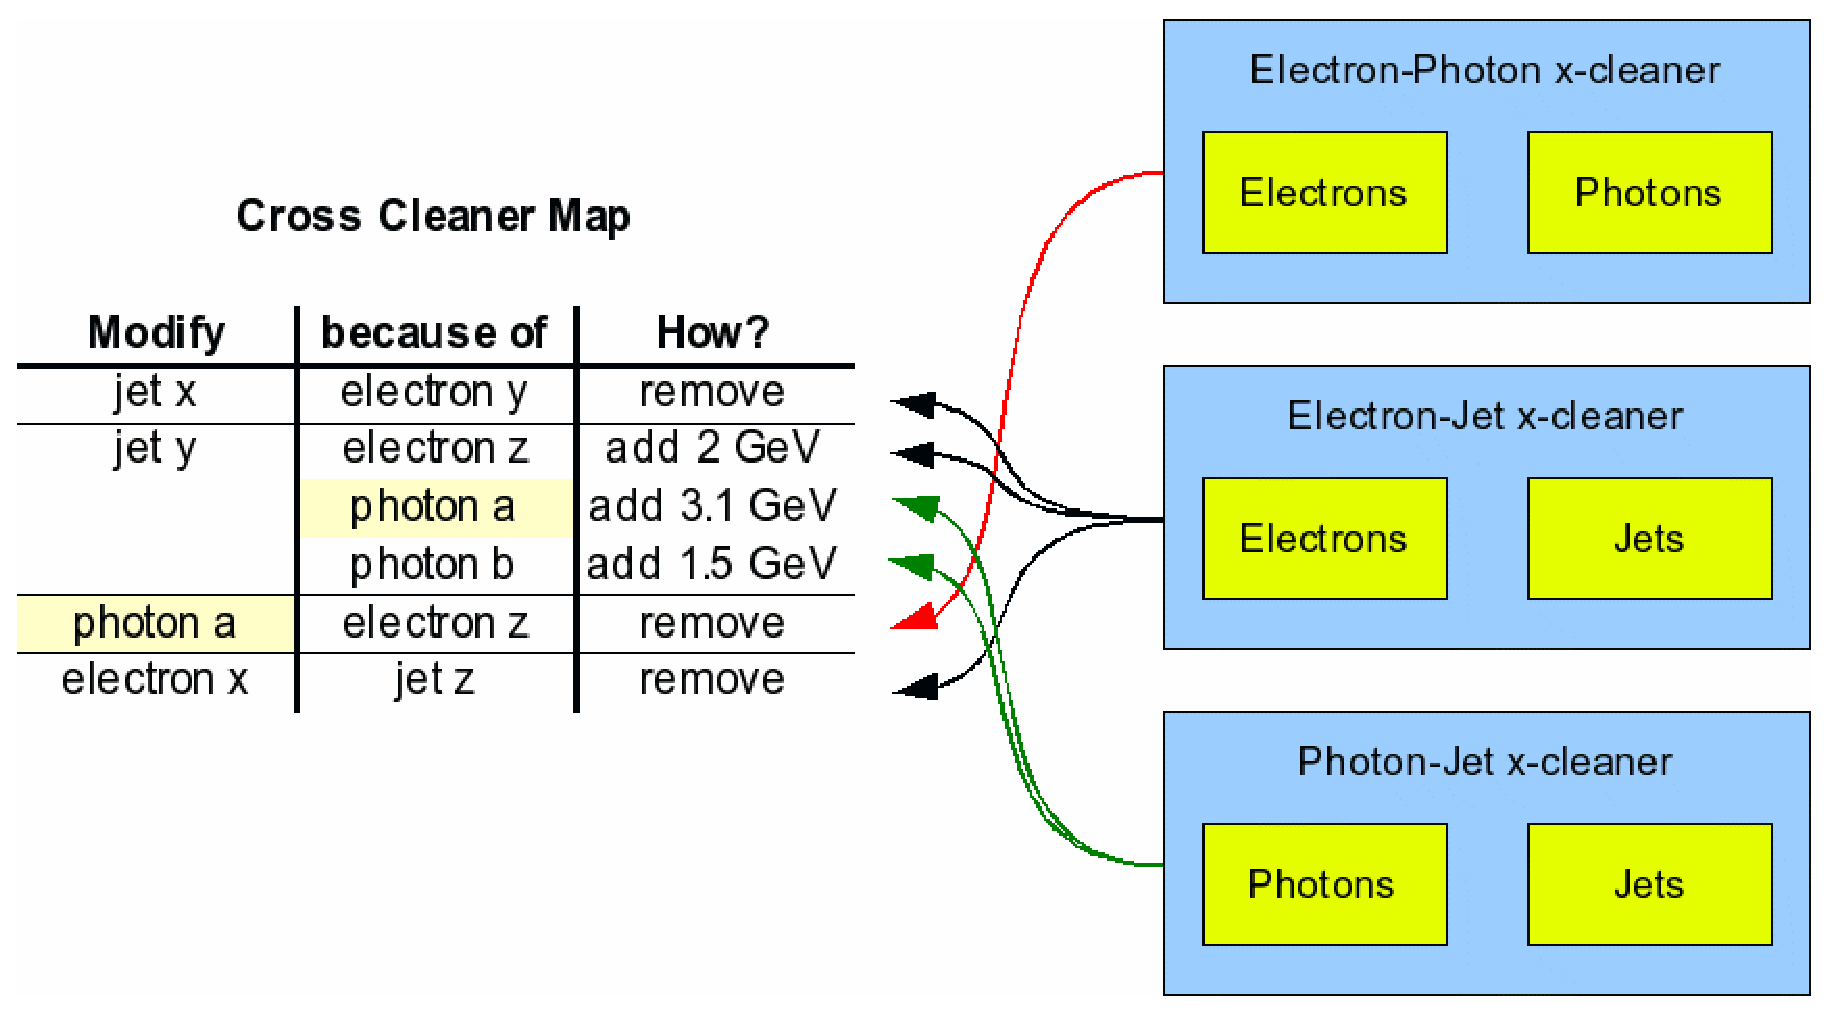
\includegraphics[scale=.4]{figures/CleaningMap.eps}
\caption{Schematic view of the input and result of different cleaning
    algorithms. Each algorithm takes two object collections as input and
    creates an entry in the internal cross-cleaning map for each object
    that should be modified.}
\label{fig:Cleaning}
\end{center}
\end{figure}
% ------------------------------------------------------------------------------

In a second step, this temporary buffer map is scanned for possible conflicts.
If the same object {\it A} is causing a correction to object {\it B} but should
be corrected itself because of object {\it C}, then it might happen that after
the correction of {\it A} the correction of {\it B} is no longer necessary or at
least different.
% to the case where first {\it B} is corrected and then {\it A}.
% right, but this case we do not take care of ...
The result of the cross-cleaning must not depend on the order in which objects
are compared, therefore conflicts are resolved before any object is being
modified (cp. section \ref{mapReso}).

Subsequently the corrections are applied to the objects. Energy corrections for
all jets in the cleaned collection are being recalculated to ensure consistency
in the calibration.

A special object in the event is the missing transverse energy (MET). The raw
MET is calculated from calorimeter towers only and will not be changed by this
cross-cleaning. However, the JES correction to the missing $E_T$ can either be
recalculated using the new collections of corrected objects as input, or by
tracking the impact of each cross-cleaning modification on the MET. This
package~\cite{package} provides a corrected MET object using the latter way.
%Both ways should give the same result and the comparison is a valuable
%cross-check. 

The cross-cleaning package is an EDM producer which creates new collections for
the cross-cleaned objects. If for a specific event no cross-cleaning has taken
place these output collections contain identical objects as the input
collections.  In addition collections of dropped objects are created, i.e. if
one object was duplicated (e.g. an electron also reconstructed as a jet) than
either object is dropped and written into a ``dropped'' collection, while the
other object remains in the cleaned output collection.

An association of the cross-cleaned PAT objects in the new collections to the
objects before cleaning is always possible by comparing the references to the
original RECO objects (via PAT object member function
\\\texttt{originalObjectRef()}). 

All parameters available for the steering of the module are listed in the
appendix. The general setup parameters and their default values can be found in
tables~\ref{tab:TurnOnModules}-\ref{tab:JetCorrections} including a short
description.

In the following sections the binary cleaners are explained in detail and their
performance is demonstrated. In section \ref{mapReso} the consistency check for
the internal map is described. In the end conclusions for the application of
this package in physics analyses on supersymmetry are drawn.

% ******************************************************************************

\section{Electron - Jet Cleaning}
\label{sec:ElecJet}
Electrons reconstruction starts from clusters in the electromagnetic calorimeter
whereas calorimeter towers used for jet clustering comprise energy in both the
hadronic and electromagnetic calorimeter. This implies that a fraction of the
ECAL energy might contribute to the reconstruction of two objects, namely an
electron and a jet. It is important to distinguish between the three cases of
\begin{enumerate}
\item  a real jet with a high electromagnetic fraction
\item an electron whose shower might have leaked into the hadronic
    calorimeter
\item an electron and a jet which are located very close together in the
    detector.
\end{enumerate}
Therefore the following procedure includes the possibilities to keep either the
jet or the electron or both objects in the event.

Starting point for this cleaning is a collection of well identified electrons.
The level of identification can be chosen from those provided by the EGamma POG
~\cite{elecID}.

The Electron-Jet cross cleaning has been tested on a variety of samples. All
plots in this section have been created from either a SUSY LM4 Sample from
Summer08 production\\
(\texttt{/SUSY\_LM4-sftsht/Summer08\_IDEAL\_V11\_redigi\_v1/GEN-SIM-RECO})\\
or a sample of
$Z\rightarrow ee$ events \\(\texttt{/Zee/Summer08\_IDEAL\_V11\_redigi\_v2/GEN-SIM-RECO}).

The PAT objects have been generated using the default sequences provided in the
configuration files\\
\texttt{PhysicsTools/PatAlgos/python/patLayer0\_cff.py} and\\
\texttt{PhysicsTools/PatAlgos/python/patLayer1\_cff.py} in the CMSSW\_2\_2\_7
release. Acceptance cuts for the pat objects as listed in
table~ref{tab:PATobjCuts} have been applied on all samples used in this study.
All other parameters have been set as listed in the appendix.

% ------------------------------------------------------------------------------
\begin{table}[h]
\caption{Cuts on PAT Layer 1 objects}
\begin{center}
\begin{tabular}{l|c|c}
\textbf{Object} & \textbf{$p_T$} & \textbf{$|\eta|$} \\ \hline
    Electrons & $>10$\,GeV & $<2.5$  \\\hline
    Muons     & $>10$\,GeV & $<2.5$  \\\hline
    Photons   & $>10$\,GeV & $<2.5$  \\\hline
    Jets      & $>15$\,GeV & $<2.5$
\end{tabular}
\end{center}
\label{tab:PATobjCuts}
\end{table}
% ------------------------------------------------------------------------------

\subsection{Algorithm}
The implemented algorithm is similar to the cleaning in a previous analysis
tool used in the SUSY PAG, the SusyAnalyzer~\cite{SusyAnalyzer}.

In very dense events as predicted for supersymmetric particle production, it is
not uncommon for an electromagnetic object to have shared energy with more than one jet (Fig. ~\ref{fig:NbJets}).

% ------------------------------------------------------------------------------
\begin{figure}[hbtp]
  \begin{center}
    \includegraphics[scale=1.0]{figures/ElecJet/LM4_no_of_nnj.eps}
    \caption{Number of Jets with shared energy for isolated (dashed line) and non-isolated (solid line) electrons in an event.}
    \label{fig:NbJets}
  \end{center}
\end{figure}
% ------------------------------------------------------------------------------

Therefore for each electron the three closest jets in \( \eta-\phi\) space are
examined. If this distance is smaller than $\Delta R=1.0$ (configurable) the
objects' constituents are compared in order to determine the amount of energy
which is being shared between the two objects.
This shared energy is calculated by adding up the electromagnetic energy of
those calorimeter towers which are covered by both objects, i.e. all jet towers
containing crystals which are part of the electrons' supercluster.
\footnote{Note that this is only an approximation to the real energy overlap. In
principle the more precise energies of individual crystals could be used for
calculation but these are not necessarily accessible in all analysis data
formats like e.g. PAT Layer 1 files.}
% Method using individual ECAL crystals 

If electron and jet share energy the further treatment depends on the isolation
of the electron. While the possible choices for the isolation algorithm include
the default PAT options like cone isolation in the Tracker, hadronic and
electromagnetic calorimeter, the presetting is a combination of these three, i.e. 
\begin{equation}
    CombRelIso=\frac{a\cdot ECalIso+b\cdot HCalIso+c\cdot TrackIso}{p_T}
    \label{ElIsolation}
\end{equation}
, with \(a=b=c=1\). This Isolation variable has been suggested by the V+jets
group~\cite{vplusjets}. Figure ~\ref{Iso} shows this combined
isolation for Electrons. The cut at \(0.1\) was also recommended in the V+jets
group baseline selection.

% ------------------------------------------------------------------------------
\begin{figure}[hbtp]
  \begin{center}
    \includegraphics[scale=0.8]{figures/ElecJet/LM4_isolation_B.eps}
    \includegraphics[scale=0.8]{figures/ElecJet/LM4_isolation_A.eps}
    \caption{Combined isolation (see eq. (~\ref{ElIsolation})) for Electrons before (left) and after (right) cross cleaning.}
    \label{fig:ElectronIsolation}
  \end{center}
\end{figure}
% ------------------------------------------------------------------------------

If it is non-isolated the electron will be removed and the difference between
the electron energy and the shared energy will be added to the jet. This energy
correction is applied vectorially. It is given by the difference of the electron
fourvector and a massless 'shared energy' fourvector.

This fourvector is calculated from the electromagnetic energy of those towers
that overlap with the electron's supercluster. For each
tower an energy vector $(E_x, E_y, E_z)$ is calculated from the electromagnetic
energy and the $\eta$ and $\phi$ coordinates. All the vectors are added
up and finally transformed into a massless fourvector ($E^2=\vec{p}^2$).

For isolated electrons we distinguish two cases. If the ratio of shared energy
and jet energy is greater than a certain value the jet will be removed. If the
ratio is smaller both objects are kept and the shared energy fourvector is subtracted from
the jet. This way objects very close in $\Delta R$ can be kept in the events
without double counting of energy.
The steps of this procedure are illustrated in figure~\ref{fig:EJCleaning}.

% ------------------------------------------------------------------------------
\begin{figure}[hbtp]
  \begin{center}
    \includegraphics[scale=.6]{figures/ElectronJetAlgo_quer.eps}
    \caption{Steps of the electron-jet cleaning.}
    \label{fig:EJCleaning}
  \end{center}
\end{figure}
% ------------------------------------------------------------------------------

% OK, now there should be s.th. concerning vectorial subtraction vs. scaling.
All cut values are configurable and are listed with their default settings in
table~\ref{tab:ElectronJetPar}.

\subsection{Results and Validation}
In this section the effect of the described procedure on electrons and jets in
the events is studied. 

\subsubsection{Cut Variables}
% (dR, shared energy, isolation) for different matches
As described in the previous section the cleaning algorithm applies cuts on
several variables concerning the electron and jet under investigation. These are
the distance of electron and jet in $\Delta R$ and their shared energy,
normalised to the jet energy. The distributions of these variables are shown
in figure~\ref{fig:dR_sE_ElecJet_iso} (isolated electrons, before and after the
cleaning) and figure ~\ref{fig:dR_sE_ElecJet_noniso} (non-isolated electrons
before cleaning) respectively. By default the CombRelIso variable is considered.

We further investigate four different classes of electron-jet pairs. The
classification is based on the matching of the reconstructed objects
to generator particles produced in the hard process. We distinguish pairs in
which both, electron, jet or none of the objects could be matched to a generated
particle. The matching algorithm provided and used in the PAT applies a $\Delta
R$ matching.

% ------------------------------------------------------------------------------
\begin{figure}[hb]
\begin{center}
    \includegraphics[scale=0.8]{figures/ElecJet/LM4_dR_iso_B.eps}
    \includegraphics[scale=0.8]{figures/ElecJet/LM4_dR_iso_A.eps}
    \includegraphics[scale=0.8]{figures/ElecJet/LM4_sharedE_iso_B.eps}
    \includegraphics[scale=0.8]{figures/ElecJet/LM4_sharedE_iso_A.eps}
    \caption{Distance \(\Delta R\) (upper row) and shared Energy, normalised to jet energy, (lower row) with the closest Jet for isolated Electrons before (left) and after (right) the cross cleaning.}
\label{fig:dR_sE_ElecJet_iso}
\end{center}
\end{figure}
% ------------------------------------------------------------------------------

% ------------------------------------------------------------------------------
\begin{figure}[hb]
\begin{center}
    \includegraphics[scale=0.8]{figures/ElecJet/LM4_dR_noniso_B.eps}
    \includegraphics[scale=0.8]{figures/ElecJet/LM4_sharedE_noniso_B.eps}
    \caption{Distance in $\Delta R$ and Shared energy divided by the jet energy of non-isolated electron and closest jet
before the cross-cleaning.}
\label{fig:dR_sE_ElecJet_noniso}
\end{center}
\end{figure}
% ------------------------------------------------------------------------------

We observe a peak at $E_{shared}/E_{Jet}=1$ for isolated as well as for
non-isolated electrons. The peak contains mostly electrons which have a matched
generated electron but no matched generated parton/jet. Clearly the energy
deposition of the electron has been reconstructed as a jet. This motivates the
use of a cut on this ratio in order to reject fake jets. The effect of the
default cut value 0.7 is illustrated in the lower row of figure~\ref{fig:dR_sE_ElecJet_iso}.

The peak of many non-isolated electrons with a generator match and large shared
energy is caused by the hard cut on the isolation value which cuts away a
non-negligible number of electrons which can be matched to a generated electron
(Fig.~\ref{fig:ElectronIsolation}). It can be reduced by loosening the isolation
requirement.

The region with lower $E_{shared}/E_{Jet}$ ration is dominated by overlaps where
only the jet could be matched to the generator information, thus indicating fake
electrons which can be removed.

\clearpage

\subsubsection{Effects of the Cleaning}

While the cleaning is aiming at a reduction of double counted energy it will non
the less effect the electron reconstruction quality as non-isolated electrons are
removed from the event. Two control quantities that can be studied on Monte
Carlo are the reconstruction efficiency and the contamination with fake
electrons. Here we define efficiency as the ratio 
\[\frac{\mathrm{No.\ of\ reconstructed\ electrons\ w\ generator\ match}}{\mathrm{No.\ of\ generated\ electrons}}\]
and contamination as
\[\frac{\mathrm{No.\ of\ reconstructed\ electrons\ w/o\ generator\ match
}}{\mathrm{No.\ of\ all\ reconstructed\ electrons}}\]
The matching is again the PAT intrinsic one. The figures presented here are not
corrected for the matching efficiency.

With the default settings provided in the appendix a significant drop of the
efficiency is observed (Fig. ~\ref{fig:effCont_elec_ElecJet}) . This corresponds
directly to the hard cut on electron isolation ($\mathrm{CombRelIso}<0.1$) which defines
the fraction of removed objects. This drop appears uniformly over the
pseudorapidity range (figure) and amounts to about 30\%.  The effect is larger
for low $p_T$ electrons which can be explained by a larger fraction failing the
identification requirements and the higher sensitivity of the relative isolation
variable for low $p_T$ objects.

% ------------------------------------------------------------------------------
\begin{figure}[hb]
\begin{center}
    \includegraphics[scale=0.8]{figures/ElecJet/LM4_efficiency_pt.eps}
    \includegraphics[scale=0.8]{figures/ElecJet/LM4_efficiency_eta.eps}
    \includegraphics[scale=0.8]{figures/ElecJet/LM4_contamination_pt.eps}
    \includegraphics[scale=0.8]{figures/ElecJet/LM4_contamination_eta.eps}
    \caption{Efficiency (upper row) and contamination (lower row) vs. transverse
    momentum (left) and pseudorapidity (right) for electrons before and after
    the cross-cleaning} \label{fig:effCont_elec_ElecJet}
\end{center}
\end{figure}
% ------------------------------------------------------------------------------

The contamination falls to a very low level of about 5\% over the entire $p_T$
range and is mostly flat in pseudorapidity. Note that the spikes at
$|\eta|=1.4$, marking the transition from barrel to endcap calorimeter, are
greatly reduced after applying the cross-cleaning on those electrons passing the
'LooseElectron' identification.

The reconstruction efficiency of the jets is not affected (Fig.
~\ref{fig:effCont_Jets_ElecJet}). The contamination however is slightly reduced
in the range up to $p_T=300$ GeV where jets have been identified as electrons in
the cleaning.
% ------------------------------------------------------------------------------
\begin{figure}[hb]
\begin{center}
    \includegraphics[scale=0.8]{figures/ElecJet/LM4_efficiency_jets_pt.eps}
    \includegraphics[scale=0.8]{figures/ElecJet/LM4_contamination_jets_pt.eps}
    \caption{Efficiency (left) and contamination (right) vs. transverse momentum
    for jets before and after the electron-jet cross-cleaning.}
\label{fig:effCont_Jets_ElecJet}
\end{center}
\end{figure}
% ------------------------------------------------------------------------------

%\subsubsection{Resolution}
The transverse momentum and pseudorapidity spectrum for the electrons are shown
in figure ~\ref{fig:objSpectra_ElecJet}. The distributions are normalised to one
and a change in shape can be observed in both of them. The number of low $p_T$
electrons is reduced after the cross-cleaning what corresponds to the observed
drop in efficiency at low $p_T$ due to identification and isolation
efficiencies. As already observed in the contamination the spikes from fake
electrons, located at the transition region from barrel to endcap calorimeter
around $|\eta|=1.4$ cleaned away.

% ------------------------------------------------------------------------------
\begin{figure}[hb]
\begin{center}
    \includegraphics[scale=0.8]{figures/ElecJet/LM4_obj_pt.eps}
    \includegraphics[scale=0.8]{figures/ElecJet/LM4_obj_eta.eps}
    \caption{Transverse momentum and pseudorapidity spectra before
    and after the electron-jet cross-cleaning.}
\label{fig:objSpectra_ElecJet}
\end{center}
\end{figure}
% ------------------------------------------------------------------------------

Of further interest in an analysis is the spectrum of the so-called recoiled
missing transverse energy (recoil met). It is calculated by adding up the
fourvectors of all objects (passing the ID) in the event, that is electrons,
muons, tau, jets, and photons (\textcolor{red}{recheck after photon ID works}).
This quantity is very sensitive to double counting of energy in the event.

The result for electron - jet cross cleaning is shown in figure
~\ref{fig:met_ElecJet} in comparison to the missing transverse energy from the
calorimeter towers, corrected for the jet energy scale (L2, L3). While they are
in good agreement at the lower energy range (up to \(\sim 500 GeV\)), the
distributions differ in the tail. The gap between 'recoil' and 'calo' missing
$E_T$ is closed by the cross-cleaner, demonstrating an effective removal of
overlaps and therefore double counting of energy.

% ------------------------------------------------------------------------------
\begin{figure}[hb]
\begin{center}
    \includegraphics[scale=0.8]{figures/ElecJet/LM4_METcomp.eps}
    \caption{Spectrum of missing transverse energy from fourvector sum of all
    particles before and after the electron-jet cross-cleaning. For comparison
    the missing $E_T$ from calorimeter towers is shown as well.}
\label{fig:met_ElecJet}
\end{center}
\end{figure}
% ------------------------------------------------------------------------------
All in all the cleaning is a reasonable addition to the
common electron ID procedure. As always one can trade efficiency for purity,
here labeled as contamination, by varying the isolation cut.

\paragraph{Zee events}
Some words here about the performance in $Z\rightarrow ee$.

\clearpage

% *** MUON-JET CLEANING ********************************************************

\section{Muon - Jet Cleaning}
The idea behind the muon-jet cleaning is to merge those muons into the jet which
are produced in this jet by decay-in-flight of b and c hadrons\footnote{The same
idea is pursued in the Jet Plus Track algorithms.}.

The user must take care not to include fake muons in the cleaning. Those can
result from punch-through of hadrons into the muon system and might have very
high transverse momentum which spoils the jet collection. An appropriate muon
identification can be chosen from the muon POG defaults~\cite{muonID}.

The Muon-Jet cross cleaning was tested on \\
\texttt{/SUSY\_LM4-sftsht/Summer08\_IDEAL\_V11\_redigi\_v1/GEN-SIM-RECO} and\\
\texttt{/Zmumu/Summer08\_IDEAL\_V11\_redigi\_v2/GEN-SIM-RECO}.

All plots in this section are obtained from the LM4 Sample using CMSSW 2.2.8. The following CVS
tags have been used on top of this release:
\begin{itemize}
    \item DataFormats/PatCandidates V03-18-09      
    \item PhysicsTools/PatAlgos     V04-14-25      
    \item PhysicsTools/PatUtils     V03-05-02      
\end{itemize}
The PAT objects
have been generated using the default sequences provided in the configuration
files\\
\texttt{PhysicsTools/PatAlgos/python/patLayer0\_cff.py} and\\
\texttt{PhysicsTools/PatAlgos/python/patLayer1\_cff.py}.

Some plots made with the Zmumu sample can be found in appendix~\ref{app:Zmumu}.


\subsection{Algorithm}
In this cross-cleaner module all non-isolated muons are considered as part of
the jet which is within a distance of $\Delta R=0.2$ . Isolation refers either
to both tracker and calorimeter or the CombRelIso variable. The muon objects are
removed and their fourvector added to the jet object. 
%(To avoid any double counting of energy we subtract the MIP
%signal of the muon in the calorimeter which is already contained in the
%jet. Still to add in the code!)
This is sketched in figure~\ref{fig:MJCleaning}.

% ------------------------------------------------------------------------------
\begin{figure}[hbt]
\begin{center}
\includegraphics[scale=.6]{figures/MuonJet/MuonJetAlgo_quer.eps}
\caption{Steps of the muon-jet cleaning.}
\label{fig:MJCleaning}
\end{center}
\end{figure}
% ------------------------------------------------------------------------------

Again the cut values on the distance and isolation are configurable (see
tab.~\ref{tab:MuonJetPar}). A switch has been introduced to turn off the
correction of the jet energy. This is meant to be used in combination with JPT
where the muon energy has already been added in the jet reconstruction but the
muon has not yet been removed.

\subsection{Validation}
\subsubsection{Cut Variables}
In the muon - jet cross cleaning the isolation is used to decide which muon is
candidate for removing and which not. Figure~\ref{fig:MuonIsolation} shows the
combined isolation as defined in eq.(~\ref{ElIsolation}) for muons before and
after the cleaning. The preset isolation cut is on \(0.1\) \(G\)e\(V\). 

% ------------------------------------------------------------------------------
\begin{figure}[hb]
\begin{center}
    \includegraphics[scale=0.8]{figures/MuonJet/LM4_iso_Muon_before.eps}
    \includegraphics[scale=0.8]{figures/MuonJet/LM4_iso_Muon_after.eps}
    \caption{Combined isolation for muons before (left) and after (right) the
    muon-jet cross cleaning.}
\label{fig:MuonIsolation}
\end{center}
\end{figure}
% ------------------------------------------------------------------------------


Then, the distance \(\delta R\) between the (non-isolated) muon and all jets in
\(\eta - \phi\) space is calculated. If there exists a jet which is closer than
a certain value (preset is \(\delta R < 0.2\)), the muon will be removed,
otherwise both muon and jets will be left alone.
Figure~\ref{fig:dR_MuonJet_noniso} shows this for before and after the cross
cleaning. As the energy correcion of the jet is a vectorial correction, it may
happen that a jet, which is not in cleaning distance of a non-isolated muon
before the cleaning, is moved into cleaning distance after the cross cleaning.
This effect can also be seen in figure~\ref{fig:dR_MuonJet_noniso}.

% ------------------------------------------------------------------------------
\begin{figure}[hb]
\begin{center}
    \includegraphics[scale=0.8]{figures/MuonJet/LM4_dR_MuonJet_noniso_before.eps}
    \includegraphics[scale=0.8]{figures/MuonJet/LM4_dR_MuonJet_noniso_after.eps}
    \caption{\(\delta R\) between non-isolated muon and jet before (left) and
    after (right) the muon-jet cross cleaning.}
\label{fig:dR_MuonJet_noniso}
\end{center}
\end{figure}
% ------------------------------------------------------------------------------

\subsubsection{Selection Efficiency and Fake Rate}
The greatest influence of muon - jet cross cleaning is on the contamination of
the muons. It drops from \(40 \%\) to \(10 \%\) with the default settings. The
selection efficiency on the other hand also decreases, but stays good (\(\sim
90\%\)). This can be seen in figure~\ref{effCont_muon_MuonJet} for the \(p_T\)
and \(\eta\) distributions. 

% ------------------------------------------------------------------------------
\begin{figure}[hb]
\begin{center}
    \includegraphics[scale=0.8]{figures/MuonJet/LM4_Eff_pt_Muon.eps}
    \includegraphics[scale=0.8]{figures/MuonJet/LM4_Eff_eta_Muons.eps}\\
    \includegraphics[scale=0.8]{figures/MuonJet/LM4_Cont_pt_Muons.eps}
    \includegraphics[scale=0.8]{figures/MuonJet/LM4_Cont_eta_Muons.eps}
    \caption{Effiency (upper row) and contamination (lower row) vs. transverse
    momentum (left) and pseudorapidity (right) for muons before and after the
    muon-jet cross-cleaning}
\label{fig:effCont_muon_MuonJet}
\end{center}
\end{figure}
% ------------------------------------------------------------------------------

Again, this cross cleaning module has nearly no impact on selection efficiency
and contamination of the jets (figure~\ref{effCont_Jets_MuonJet}).

% ------------------------------------------------------------------------------
\begin{figure}[hb]
\begin{center}
    \includegraphics[scale=0.8]{figures/MuonJet/LM4_Eff_pt_Jets.eps}
    \includegraphics[scale=0.8]{figures/MuonJet/LM4_Cont_pt_Jets.eps}
    \caption{Effiency (left) and contamination (right) vs. transverse momentum
    for jets before and after the muon-jet cross-cleaning.}
\label{fig:effCont_Jets_MuonJet}
\end{center}
\end{figure}
% ------------------------------------------------------------------------------

\subsubsection{Resolution}
As shown in the \(p_T\) spectrum of the muons in
figure~\ref{fig:ObjSpectra_MuonJet} (left), the cross cleaning effects mainly
the soft muons, located more centrally in terms of pseudorapidity (right).

% ------------------------------------------------------------------------------
\begin{figure}[hb]
\begin{center}
    \includegraphics[scale=0.8]{figures/MuonJet/LM4_Spectrum_Muon_pt.eps}
    \includegraphics[scale=0.8]{figures/MuonJet/LM4_Spectrum_Muon_eta.eps}
    \caption{\(p_T\) (left) and \(\eta\) (right) spectra for muons before and
    after the muon-jet cross cleaning.}
\label{fig:ObjSpectra_MuonJet}
\end{center}
\end{figure} 
% ------------------------------------------------------------------------------

On the recoil met, defined as in section~\ref{sec:ElecJet}, the muon-jet cross
cleaning has nearly no effect (see fig~\ref{fig:met_MuonJet}).

% ------------------------------------------------------------------------------
\begin{figure}[hb]
\begin{center}
    \includegraphics[scale=0.8]{figures/MuonJet/LM4_met_MuonJet.eps}
    \caption{Spectrum of missing transverse energy from fourvector sum of all
    particles before and after the muon-jet cross cleaning. For comparison the
    missing $E_T$ from calorimeter towers is shown as well.}
\label{fig:met_MuonJet}
\end{center}
\end{figure}
% ------------------------------------------------------------------------------

\clearpage

% ******************************************************************************

\section{Photon - Jet Cleaning}
In the CMS default reconstruction photons are selected with rather loose criteria
from all reconstructed superclusters in the event. Like in the case of electrons
an adequate photon identification must be applied in order to remove fake and/or
non-isolated photons. Any photon entering the cross-cleaning must fulfill the
requirements of a certain identification, which can be chosen from the ones
deployed by the EGamma POG (put a reference here). 

Again the energy deposit in the supercluster might also be part of a
calorimeter tower and thus be used in jet reconstruction. These ambiguities in
the assignment of energy to the objects are resolved in a scheme similar to the
electron-jet disambiguation described in section~\ref{sec:ElecJet}. 
%Note that the jet is only removed if it shares its entire energy with a photon
%% NOT ANY MORE
(cp.~fig.~\ref{fig:PJCleaning}).

%\subsection{Algorithm}

% ------------------------------------------------------------------------------
\begin{figure}[hbt]
\begin{center}
\includegraphics[scale=.6]{figures/PhotonJetAlgo_quer.eps}
\caption{Steps of the photon-jet cleaning.}
\label{fig:PJCleaning}
\end{center}
\end{figure}
% ------------------------------------------------------------------------------

\subsection{Validation}

% ******************************************************************************

\clearpage
\section{Electron - Photon Cleaning}
Both kinds of objects are reconstructed from superclusters in the
electromagnetic calorimeter. Before object identification procedures are applied
the electron collection is just a subset of the photon collection (put a
reference here) with the additional requirement that a track matches the
supercluster. For disambiguation it is necessary to remove those photons which
share the supercluster seed or even supercluster with a good electron.
Therefore the reference to the supercluster (seed) of all electron-photon pairs
in the event are compared and duplicates are removed from the photon collection
(Fig.~\ref{fig:EPCleaning}). The electron collection is not affected by this
module. This module does not have configurable parameters.

% ------------------------------------------------------------------------------
\begin{figure}[hbt]
\begin{center}
\includegraphics[scale=.6]{figures/ElectronPhotonAlgo_quer.eps}
\caption{Steps of the electron-photon cleaning.}
\label{fig:EPCleaning}
\end{center}
\end{figure}
% ------------------------------------------------------------------------------

\subsection{Validation}
\clearpage

% *** CONCLUSIONS **************************************************************

\section{Combined Cleaning}
For an optimal cleaning in an analysis considering several or all of the
different objects the discussed parts can be used simultaneously. The individual
cleaners are run one after the other, all adding information to the internal
map. After that the map is checked for consistency (cp.~\ref{mapReso}).
In this section the performance of the cross-cleaner in this full feature mode
is shown. \ldots once we have the plots.

\section{Resolving Conflicts}
\label{mapReso}
All overlaps detected in the comparison of collections among each other are
being stored in an association map as described above. The next step in the cleaning procedure
consists of finding contradictions in this map and resolving them.
Possible configurations needing such an intervention are
\begin{enumerate}
    \item Object A is marked to be \textit{deleted} because of overlap with
	object B and marked for \textit{modification} due to a conflict with
	object C
    \item Object A is marked to be \textit{deleted} because of overlap with object B
	which itself is marked for deletion due to a conflict with object C.
%    \item Object A is marked to be \textit{modified} because of overlap with object B
%	which itself is marked for deletion due to a conflict with object C.
%	NOT YET RESOLVED AND RATHER IMPOSSIBLE DUE TO STRUCTURE OF THE MAP
    \item A closed loop of dependencies (Fig.~\ref{fig:loopReso}) % To be created
\end{enumerate}

% Explain how this can occur, examples
% ------------------------------------------------------------------------------
\begin{figure}[hb]
\begin{center}
    \includegraphics[scale=0.4]{figures/loopConflict.eps}
    \hspace*{1.5cm}
    \includegraphics[scale=0.4]{figures/loopConflictResolved.eps}
    \caption{Circular dependencies in the cross-cleaning before the 
    consistency check of the map and cleared structure without a loop
    afterwards. The arrow points toward the object which is removed in the
    cleaning.}
    \label{fig:loopReso}
\end{center}
\end{figure}
% ------------------------------------------------------------------------------

The first case is being handled at the point where the clean collections are
being created. The action of deletion gets priority over all other
modifications.

In order to find conflicts of the other kinds all map entries are inspected. For
each entry those modifier objects leading to a deletion are checked whether they
appear themselves in the map as a modified object marked for deletion. If this
is the case a conflict of type 2 has been found. As a consequence the initial
action (removal of object A)  should not take place and the corresponding
modifier (object B) is removed from the list of modifier objects.

For the detection of a loop of dependencies not only the modifiers of the
starting object must be checked but iteratively all the modifiers' modifier. A
bookkeeping of all objects appearing in the procedure allows the detection of
the loop.

Once a loop has been detected some modifications to the map become necessary.
The idea is to keep the most energetic object of the loop (the highest in
$p_T$). Therefore the list of modifiers of this kept object is cleared off by
removing all other objects appearing in the loop. % IS THIS REALLY DONE? CHECK!
The same is done for these other objects but in addition the kept object is
added as a modifier marking them for deletion. The new topology is also sketched in
figure~\ref{fig:loopReso}.

\clearpage
\section{Conclusions}
% Default parameters

% *** DOCUMENTATION ************************************************************

\clearpage
\section{Documentation}
Up-to-date instructions how to obtain the code, compile and run it, and use its
output are maintained on a CMS wiki page~\cite{twiki}. Examples on how to
configure the package are linked from this page. New versions of the package are
advertised on the page on SUSY specific PAT extensions~\cite{susypat}.

%% Generate doxygen documentation => Ask top people how to do this.

% Internal structure/code details/How to modify the cleaner?
% Section code structure?

% *** USER VALIDATION **********************************************************

\clearpage
\section{User Validation}
The CMSSW module and a set of configuration files and ROOT scripts used to
generate the plots in this note are available on CVS. Instructions on how to use
them can be found on the wiki page~\cite{twiki}.

% *** APPENDIX - CONFIG PARAMETERS *********************************************

\clearpage
\begin{appendix}
\section{Configurable Parameters}
% ------------------------------------------------------------------------------
\begin{table}[h]
\caption{Turning on and off the components}
\begin{center}
\begin{tabular}{l|l|l|l}
\textbf{Type} & \textbf{Name} & \textbf{Description} & \textbf{Default
    Setting} \\ \hline
    bool & doElectronJetCC   & Turn on/off electron-jet cleaning & True
    \\\hline
    bool & doPhotonJetCC     & Turn on/off photon-jet cleaning  & False
    \\\hline
    bool & doMuonJetCC       & Turn on/off muon-jet cleaning     & True
    \\\hline
    bool & doElectronPhotonCC& Turn on/off electron-photon cleaning & True
\end{tabular}
\end{center}
\label{tab:TurnOnModules}
\end{table}
% ------------------------------------------------------------------------------

% ------------------------------------------------------------------------------
\begin{table}[h]
\caption{Choosing the input collections}
\begin{center}
\begin{tabular}{l|l|l|l}
\textbf{Type} & \textbf{Name} & \textbf{Description} & \textbf{Default
Setting} \\ \hline
InputTag & patJets      & Input jet collection   & selectedLayer1Jets
\\\hline
InputTag & patMets      & Input MET collection   & selectedLayer1METs
\\\hline
InputTag & patMuons     & Input muon collection  & selectedLayer1Muons
\\\hline
InputTag & patElectrons & Input electron collection &
selectedLayer1Electrons 
\\\hline
InputTag & patPhotons   & Input photon collection& selectedLayer1Photons
%\\\hline
%InputTag & patTaus      & Input tau collection   & selectedLayer1Taus
\end{tabular}
\end{center}
\label{tab:InputCollections}
\end{table}
% ------------------------------------------------------------------------------
% WHAT ABOUT CALO TOWER COLLECTION? IS IT STILL USED?

% ------------------------------------------------------------------------------
\begin{table}[h]
\caption{Jet Corrections}
\begin{center}
\begin{tabular}{l|l|l}
\textbf{Type} & \textbf{Name} & \textbf{Default Setting}       \\\hline
string &L1JetCorrector       & "none"                          \\\hline 
string & L2JetCorrector      & "L2RelativeJetCorrectorIC5Calo" \\\hline
string & L3JetCorrector      & "L3AbsoluteJetCorrectorIC5Calo" \\\hline
string & L4JetCorrector      & "none"                          \\\hline
string & L5udsJetCorrector   & "none"                          \\\hline
string & L5gluonJetCorrector & "none"                          \\\hline
string & L5cJetCorrector     & "none"                          \\\hline
string & L5bJetCorrector     & "none"                          \\\hline
string & L6JetCorrector      & "none"                          \\\hline
string & L7udsJetCorrector   & "L7PartonJetCorrectorIC5qJet"   \\\hline
string & L7gluonJetCorrector & "L7PartonJetCorrectorIC5gJet"   \\\hline
string & L7cJetCorrector     & "L7PartonJetCorrectorIC5cJet"   \\\hline
string & L7bJetCorrector     & "L7PartonJetCorrectorIC5bJet" 
\end{tabular}
\end{center}
\label{tab:JetCorrections}
\end{table}
% ------------------------------------------------------------------------------

% ------------------------------------------------------------------------------
\begin{table}[h]
\caption{Parameters for electron-jet cleaning}
\begin{center}
\begin{tabular}{l|l|l|l}
\textbf{Type} & \textbf{Name} & \textbf{Description} & \textbf{Default
Setting}                                                            \\\hline
double & deltaR\_min       &
\begin{minipage}[t]{8cm}Check for overlaps within a cone of this size around
    the electron \\
\end{minipage} & 1.0                                               \\\hline
double & SharedEtoJetE     &
\begin{minipage}[t]{8cm} Ratio of shared energy to jet energy. Used for
    decision whether to drop the jet if the electron is isolated
\end{minipage} & 0.7                                                \\\hline
double & IsoValueCut       & Cut on isolation & 0.1                 \\\hline
%double & SharedEForNIsoEle & 
%\begin{minipage}[t]{8cm}Lower energy threshold for non-isolated electrons to
%    be merged into a jet
%\end{minipage} & -1.  (disabled)                                    \\\hline
string & IsolationKey      &
\begin{minipage}[t]{8cm} Key to choose isolation method as defined in
    DataFormats/PatCandidates/interface/Isolation.h\\
    The combined relative isolation recommended by the V+jets group can be
    selected as ``CombRelIso''
\end{minipage} & ``CombRelIso''                                        \\\hline
string & ElectronID        &
\begin{minipage}[t]{8cm}Key to choose cut-based identification method. Valid
    choices are: eidLoose, eidRobustHighEnergy, eidRobustLoose,
    eidRobustTight, eidTight. The names correspond to the modules defined by
    the EGamma POG in
    RecoEgamma/ElectronIdentification/python/ electronIdSequence\_cff.py\\
\end{minipage} & ``eidLoose''   \\\hline
double & ecalIsoWeight & Weight of ecal isolation in CombRelIso variable & 1.0 \\\hline
double & hcalIsoWeight & Weight of hcal isolation in CombRelIso variable & 1.0 \\\hline
double & trkIsoWeight  & Weight of tracker isolation in CombRelIso variable & 1.0
\end{tabular}
\end{center}
\label{tab:ElectronJetPar}
\end{table}
% ------------------------------------------------------------------------------

% ------------------------------------------------------------------------------
\begin{table}[h]
\caption{Parameters for muon-jet cleaning}
\begin{center}
\begin{tabular}{l|l|l|l}
\textbf{Type} & \textbf{Name} & \textbf{Description} & \textbf{Default
    Setting} \\ \hline
    double & deltaR\_min &
    \begin{minipage}[t]{8cm}Check muons within a cone of this size around
	the jet.
    \end{minipage}                                           & 0.2 \\\hline
    double & caloIso\_max    & Cut on calorimeter isolation. & 10.0\\\hline
    double & trackIso\_max   & Cut on track isolation.       & 10.0\\\hline
    string & MuonID          & 
    \begin{minipage}[t]{8cm} Key to choose identification method. All
	possible choices are defined in
	DataFormats/MuonReco/interface/Muon.h. The MuonAnalysis page
	provides more information on these methods. In case of an invalid
	parameter choice the 'AllGlobalMuons' are used. \\
    \end{minipage}                             & ``GlobalMuonPromptTight''\\\hline
    bool   & modifyJetEnergy &
    \begin{minipage}[t]{8cm} Add energy of the muon to the overlapping jet.
	Should be set to false for the use with JPT.\\
    \end{minipage}                                            & True\\\hline
    bool   & useCombRelIso   & 
    \begin{minipage}[t]{8cm}
      will use the combined isolation variable defined by the V+jets group
      instead of caloIso\_max or trackIso\_max
    \end{minipage}                                            & True\\\hline
    double & IsoValueCut     & Cut on CombRelIso              & 0.1\\\hline
    double & ecalIsoWeight   & 
    \begin{minipage}[t]{8cm}
      Weight of ecal isolation in CombRelIso variable
    \end{minipage}                                            & 1.\\\hline
    double & hcalIsoWeight   & 
    \begin{minipage}[t]{8cm}
      Weight of hcal isolation in CombRelIso variable
    \end{minipage}                                            & 1.\\\hline
    double & trkIsoWeight    & 
    \begin{minipage}[t]{8cm}
      Weight of tracker isolation in CombRelIso variable
    \end{minipage}                                            & 1.
\end{tabular}
\end{center}
\label{tab:MuonJetPar}
\end{table}
% ------------------------------------------------------------------------------

% ------------------------------------------------------------------------------
\begin{table}[h]
\caption{Parameters for photon-jet cleaning}
\begin{center}
\begin{tabular}{l|l|l|l}
\textbf{Type} & \textbf{Name} & \textbf{Description} & \textbf{Default
Setting}                                                            \\\hline
double & deltaR\_min       &
\begin{minipage}[t]{8cm}Check for overlaps within a cone of this size around
    the photon \\
\end{minipage} & 0.5                                               \\\hline
double & IsoValueCut       & Cut on isolation & 10.                 \\\hline
string & IsolationKey      &
\begin{minipage}[t]{8cm} Key to choose isolation method as defined in
    DataFormats/PatCandidates/interface/Isolation.h\\
\end{minipage} & ``CaloIso''                                        \\\hline
double & SharedEtoJetE     &
\begin{minipage}[t]{8cm} Ratio of shared energy to jet energy. Used for
    decision whether to drop the jet if the photon is isolated
\end{minipage} & 0.7                                                \\\hline
string & PhotonID        &
\begin{minipage}[t]{8cm}Key to choose cut-based identification method. Valid
    choices are: LooseEM, LoosePhoton, TightPhoton or 'none'. For further
    information see the Photon ID wiki page~\cite{photonID}
\end{minipage} & ``LooseEM''  
\end{tabular}
\end{center}
\label{tab:PhotonJetPar}
\end{table}
% ------------------------------------------------------------------------------

% ------------------------------------------------------------------------------
\clearpage
\section{Muon-Jet Cross Cleaning on Z->mumu}
\label{app:Zmumu}

\begin{figure}[hb]
\begin{center}
    \includegraphics[scale=0.8]{figures/MuonJet/LM4_Eff_pt_Muon.eps}
    \includegraphics[scale=0.8]{figures/MuonJet/LM4_Eff_eta_Muons.eps}\\
    \includegraphics[scale=0.8]{figures/MuonJet/LM4_Cont_pt_Muons.eps}
    \includegraphics[scale=0.8]{figures/MuonJet/LM4_Cont_eta_Muons.eps}
    \caption{Effiency (upper row) and contamination (lower row) vs. transverse
    momentum (left) and pseudorapidity (right) for muons before and after the
    muon-jet cross-cleaning, done on a \(Z\rightarrow\mu\mu\) sample.
    {\color{red}Platzhalter!}}
    \label{fig:effCont_muon_MuonJet_Zmumu}
\end{center}
\end{figure}

\begin{figure}[hb]
\begin{center}
    \includegraphics[scale=0.8]{figures/MuonJet/LM4_Eff_pt_Muon.eps}
    \caption{Muon multiplicity before and after the muon-jet cross-cleaning,
    done on a \(Z\rightarrow\mu\mu\) sample.{\color{red}Platzhalter!}}
    \label{fig:muon_mult_MuonJet_Zmumu}
\end{center}
\end{figure}


% ------------------------------------------------------------------------------

\end{appendix}

% *** BIBLIOGRAPHY *************************************************************
\pagebreak
\begin{thebibliography}{9}
\bibitem {package} {\bf The CVS code repository},
\underline{http://cmssw.cvs.cern.ch/cgi-bin/cmssw.cgi/UserCode/SusyAnalysis/PatCrossCleaner/}

\bibitem {twiki} {\bf Cross-cleaning package online documentation},
\underline{https://twiki.cern.ch/twiki/bin/view/CMS/SusyPatCrossCleaner/}

\bibitem {SusyAnalyzer} {\bf SusyAnalyzer online documentation}
\underline{https://twiki.cern.ch/twiki/bin/view/CMS/SusyAnalyzer}

\bibitem {susypat} {\bf SUSY PAT online documentation},
\underline{https://twiki.cern.ch/twiki/bin/view/CMS/SusyPat/}

\bibitem{muonID} {\bf Muon Identification in CMS}, CMS AN-2008/098 

\bibitem{elecID} {\bf A cut based method for electron identification in CMS}, CMS AN-2008/082 

\bibitem{photonID} {\bf Photon ID Analysis online documentation} 
\underline{https://twiki.cern.ch/twiki/bin/view/CMS/PhotonIDAnalysis}

\bibitem {vplusjets} {\bf V+Jets Cross-PAG online documentation},
\underline{https://twiki.cern.ch/twiki/bin/view/CMS/VplusJets}

\end{thebibliography}

% ******************************************************************************

\end{document}
